\subsection{Doug Healy}

I am starting my second year in work towards my PhD in Engineering Security, studying under Dr. Bloom. I received my Masters in Information Security Policy and Management (MSISPM) from Carnegie Mellon in 2013, and my BS in Electrical Engineering Technology back in 2003 from the Rochester Institute of Technology (RIT). 

I am a avid and active supporter of Scouts BSA, volunteering much of my time in support of the program, both at the Scout (11 to 18 years old) and Cub Scout (5-11 years old) levels. Being an Eagle Scout myself, I highly believe in the values and qualities it instills in our young men and women and work very hard to make the programs successful and FUN!  

For this course, I hope to become more efficient in my research. I have spent many, many hours over the summer pouring over search results from both Google Scholar and the UCCS Library. I want to learn how to hone search results, use the correct resources, to efficiently find what I am actually looking for, not what some search engine "thinks" I am looking for. This will also require me to refine how I choose my search terms.  

Secondly, I want to learn how to effectively learn to use my time in reading a scholarly document. I am not a good "skimmer" of documents or books; never have been. I want to learn how to do this more effectively and to make sure I am not missing anything. I always think I am missing important things on the page, and I want to ensure that through my skimming, I am not.   

\subsection{My Picture: }
\begin{figure}[htp]
    \centering
    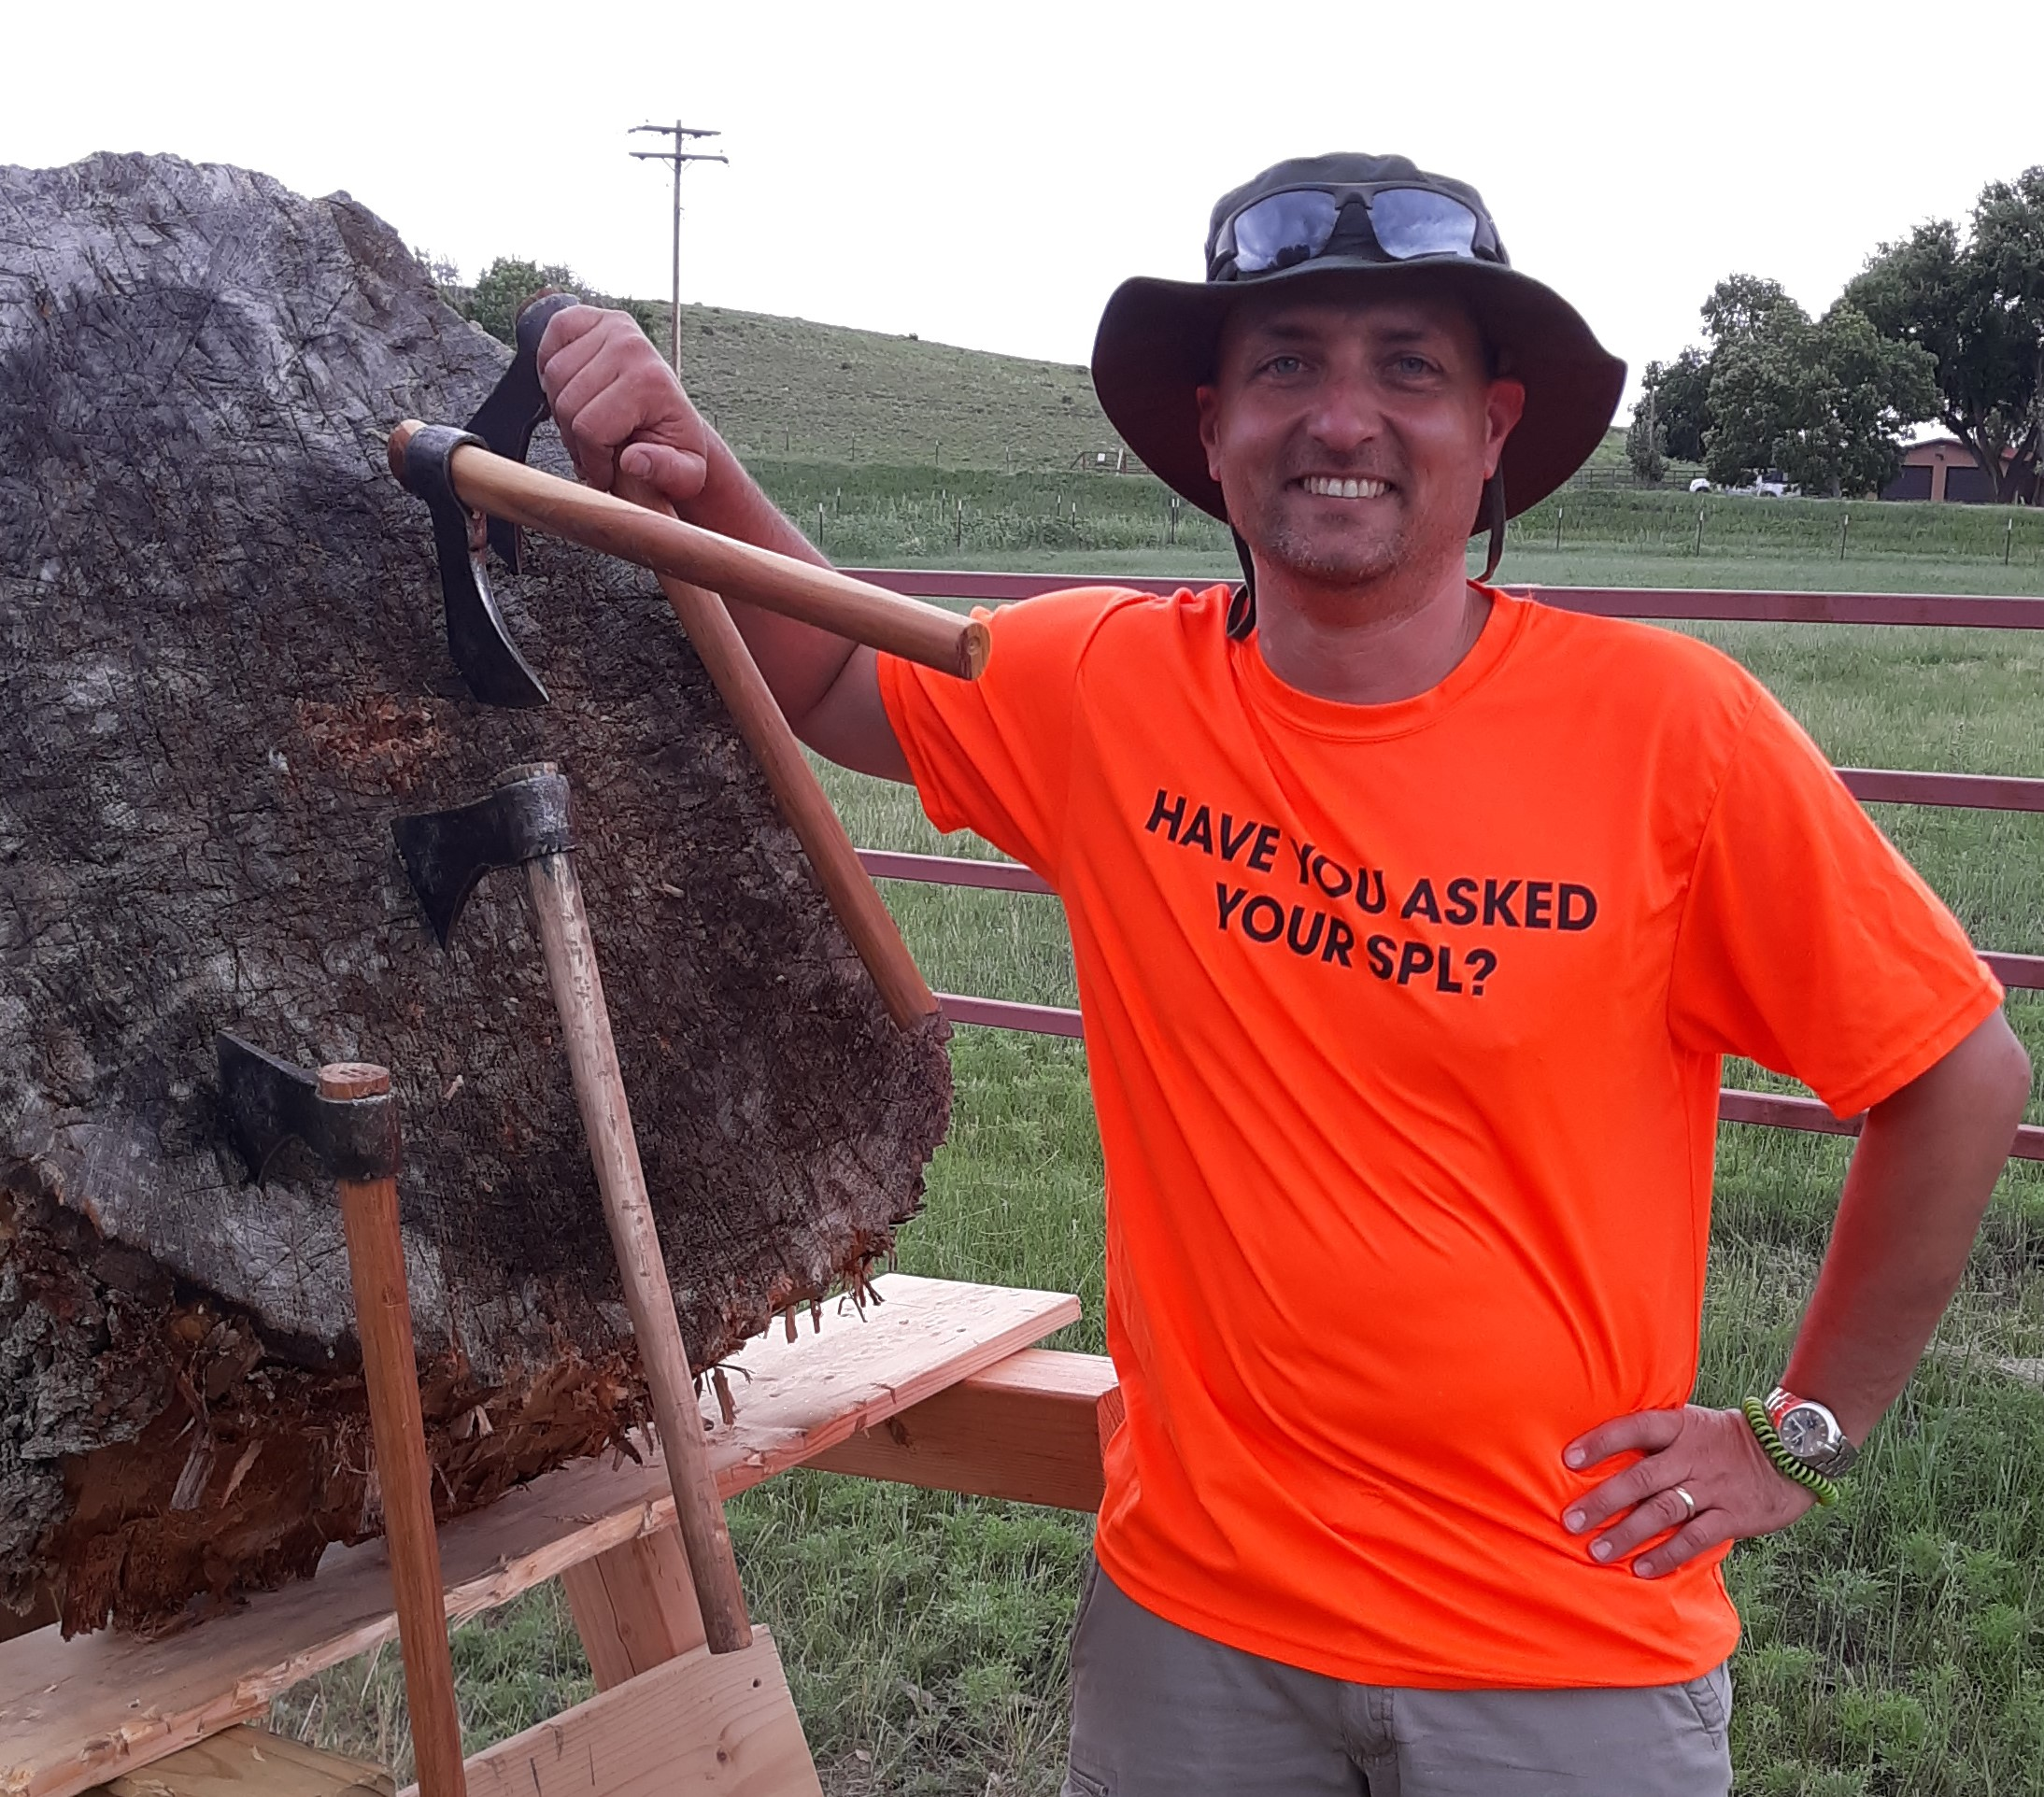
\includegraphics[scale=.095]{Healy.jpg}
    \caption{Doug Healy at Philmont Scout Ranch, Cimarron NM}
 \end{figure}
 
\subsection{Related GiT repository}
First, thanks to Will for making a comment about this! I would have missed it too...

\url{https://github.com/stamparm/tsusen} 

This repo has code for a software defined situational awareness sensor for networks. It monitors outside traffic and and logs it data into a csv file that can then be analyzed for "spikes" in traffic and predictors of malicious intent. It flushed the csv periodically and I will need to look into it more to see how often it does that.

\subsection{Q \& A}
    \begin{enumerate}
        \item AN: How was your experience at Carnegie Mellon? I was always curious about going there myself.

        \item Carnegie Mellon was great! The ISPM program was much less intense than CMU's CS department/degrees. I really enjoyed being downtown Pittsburg for the year and a half I was there. The professors were very knowledgeable, most worked at CERT or the SEI so picking their brains on what they could tells us was beneficial (due to the work space there was a LOT they couldn't tell us..). Classes were a bit more intense and we had "mini's", or half semester classes that flew by and you HAD to keep up. If you want to talk more offline or have more specifc questiosn (my knowledge is 7 years old though) send me an email and we can chat more!
    
    \end{enumerate}
